\begin{figure}
    \centering
    \begin{subfigure}[b]{0.4\textwidth}
        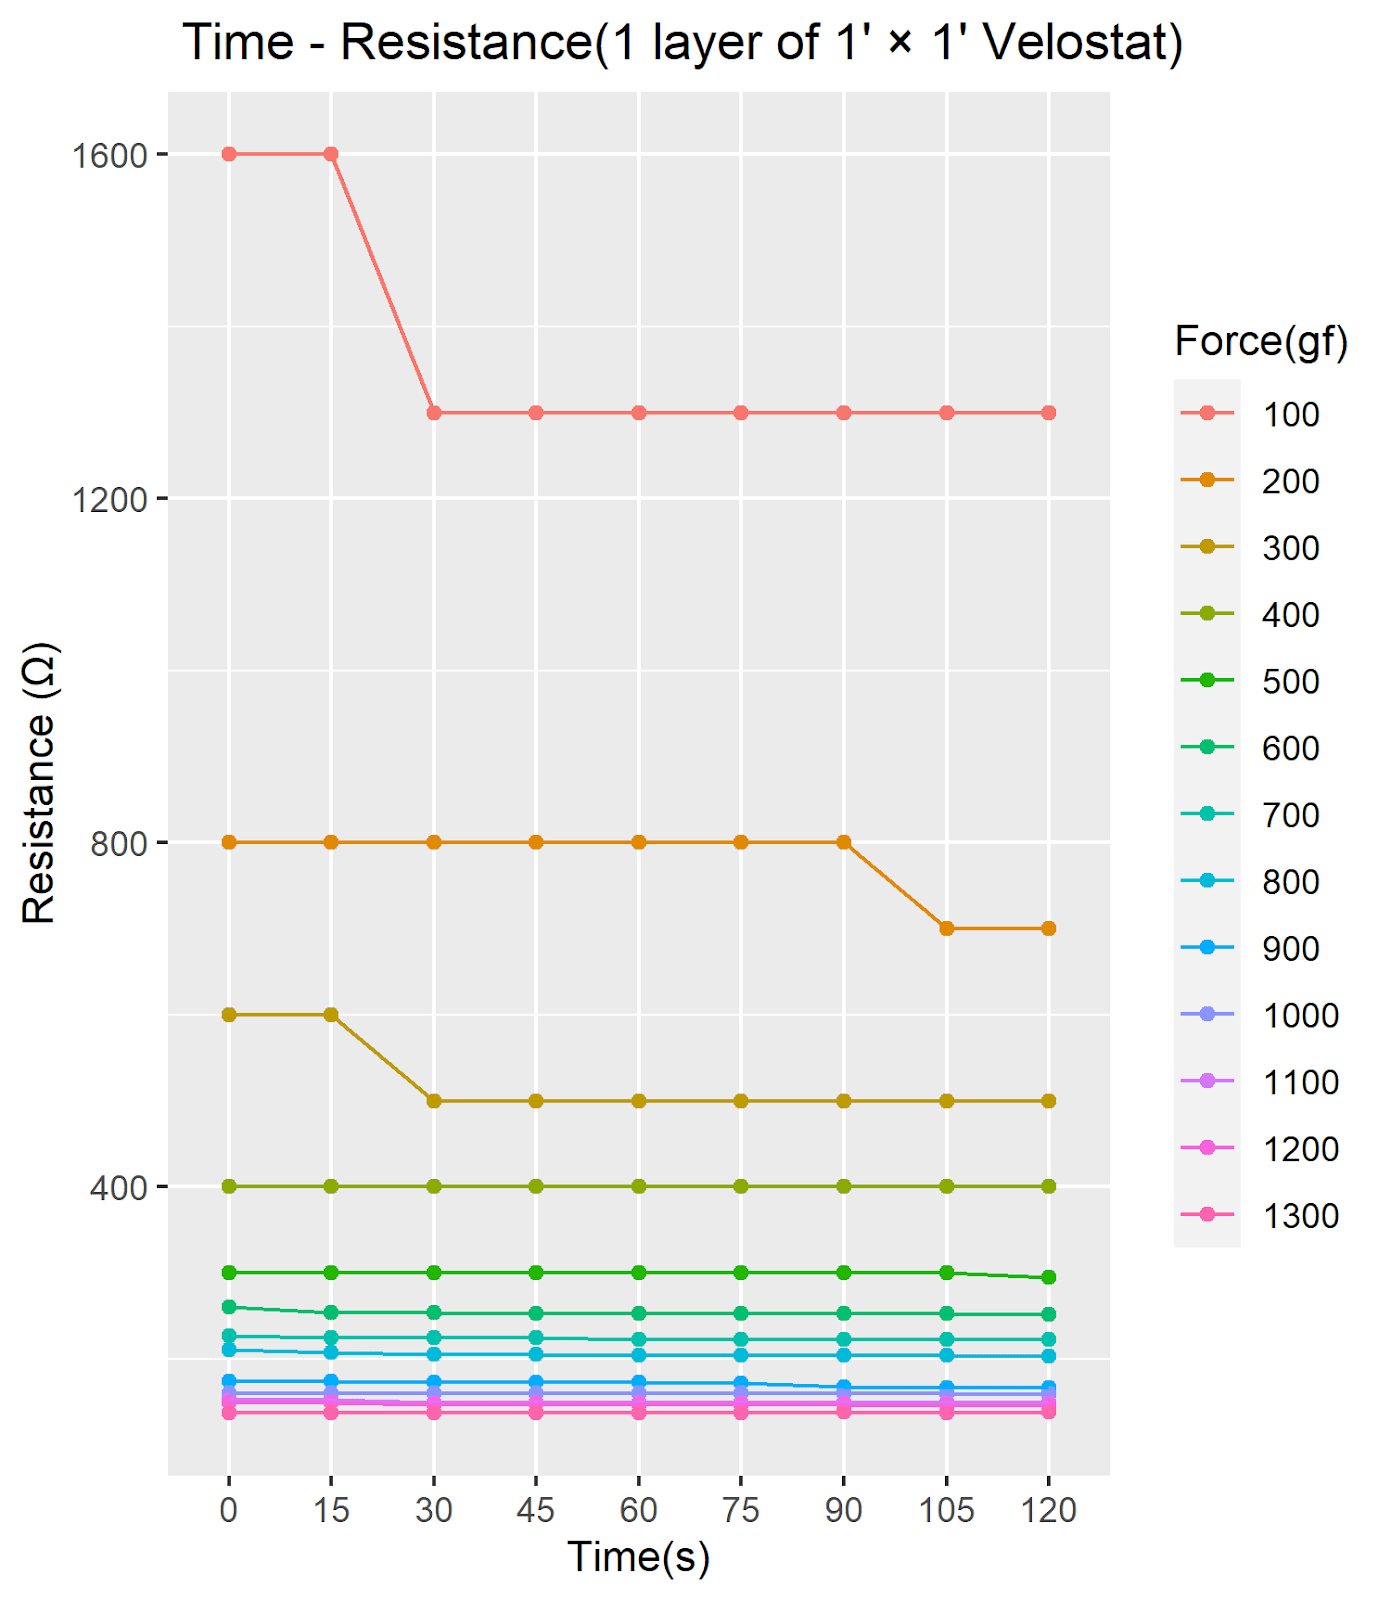
\includegraphics[width=\textwidth]{figs/one_layer.png}
        \caption{One layer of Velostat}
        \label{fig:one_layer}
    \end{subfigure}
    ~ %add desired spacing between images, e. g. ~, \quad, \qquad, \hfill etc. 
      %(or a blank line to force the subfigure onto a new line)
    \begin{subfigure}[b]{0.4\textwidth}
        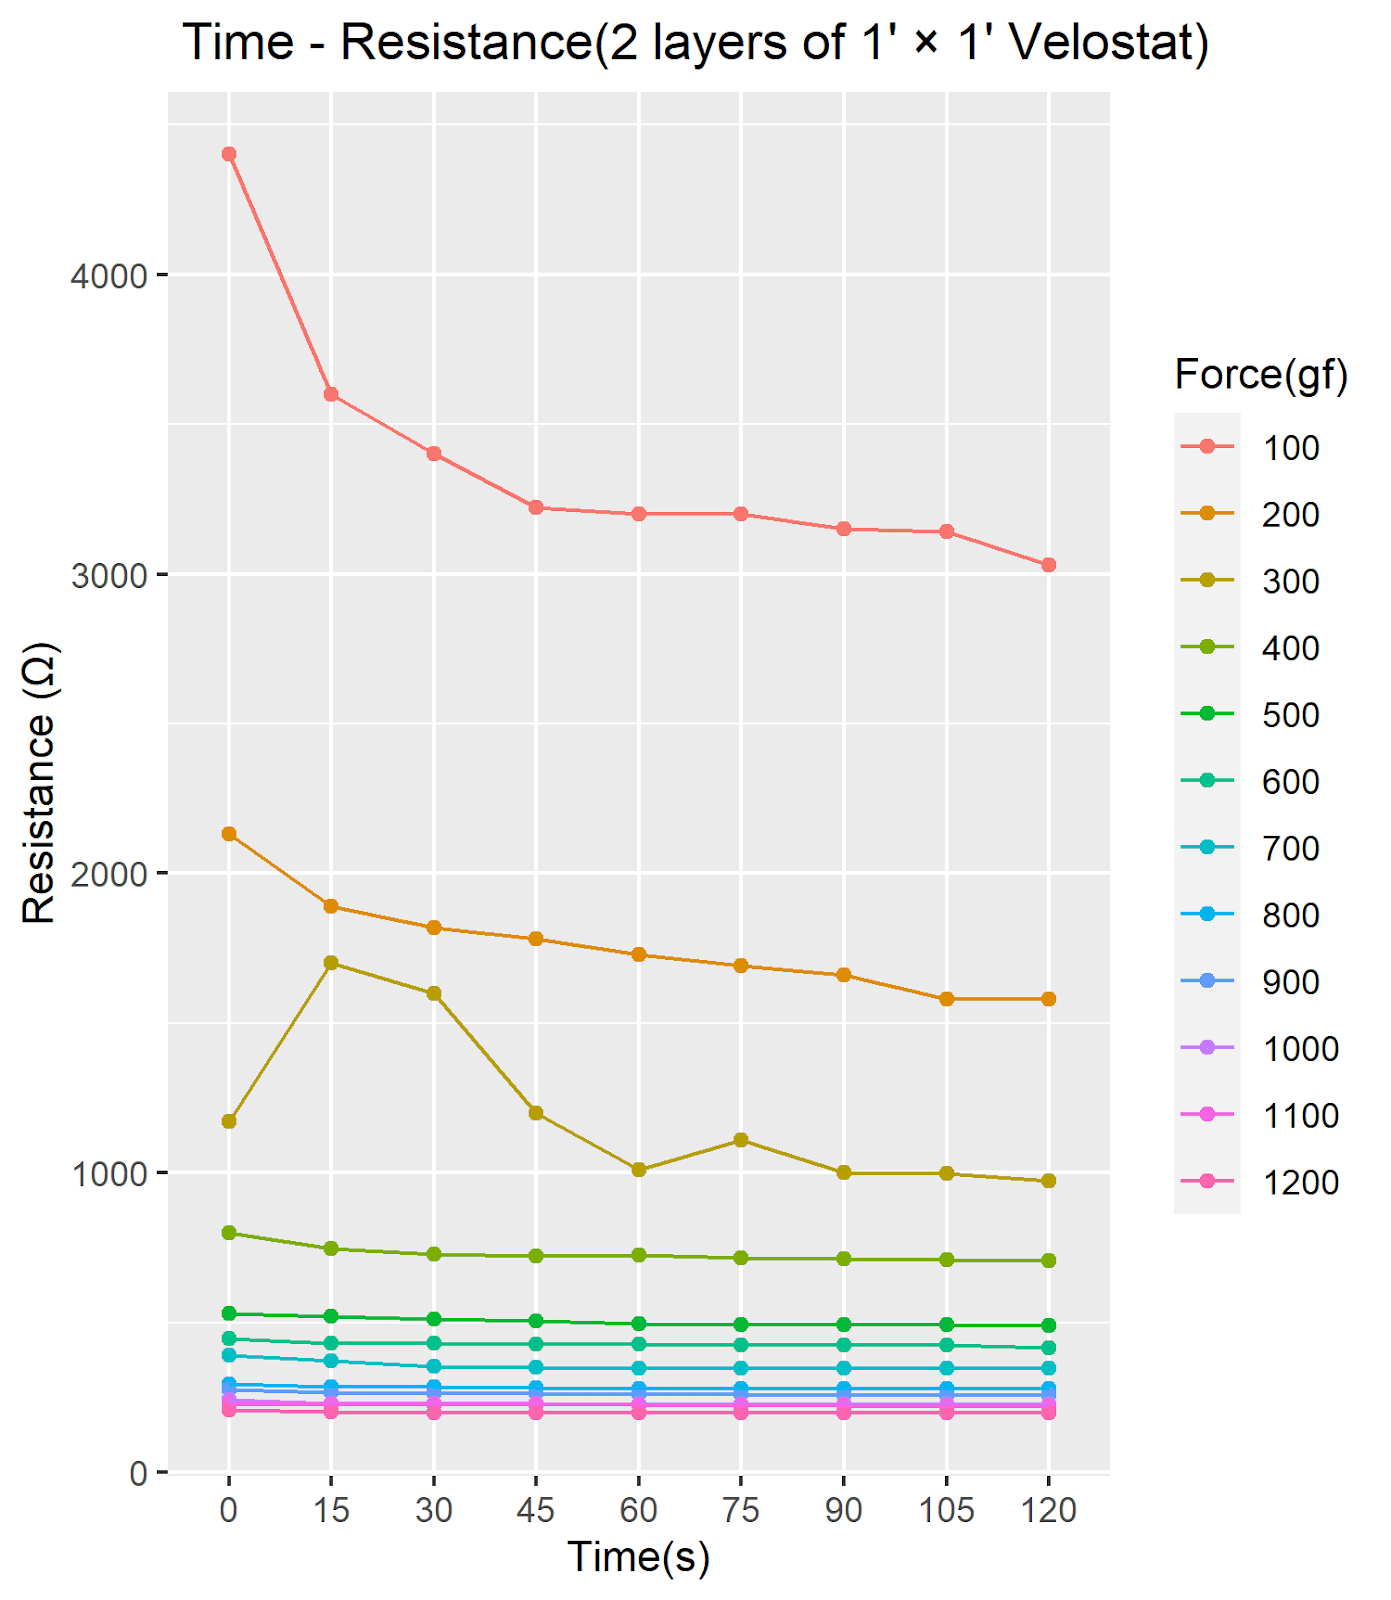
\includegraphics[width=\textwidth]{figs/two_layer.png}
        \caption{Two layers of Velostat}
        \label{fig:two_layer}
    \end{subfigure}
    \hfill %add desired spacing between images, e. g. ~, \quad, \qquad, \hfill etc. 
    %(or a blank line to force the subfigure onto a new line)
    \vspace{0.2cm}
    \caption[Compare No. of Layers]{Time for stable resistance value was higher in the case of two layers than one layer}\label{fig:hysterisis}
\end{figure}
